%!TEX root = ../dokumentation.tex

% -------------------------------
\chapter{Implementation} % ~6–7 pages, ~2400–2800 words
% -------------------------------
\label{chap:implementation}

In this chapter the implementation process of the \ac{UI} and the related logic of the full stack web application get explained. 
First, the overall architecture gets explained. Afterwards, the implementation of the frontend gets explained. Lastly, the integration with the \ac{API} backend gets outlined. 

% TODO add introduction as soon as when i know what will be in this chapter lol

\section{Overall Architecture}
Figure~\ref{fig:architecture} shows the applications' infrastructure. 
The backend is able to include multiple \ac{ASTRA-Sim} versions by building them from inside the container. The \ac{API} gets a copy of the built version and can use it from that point on. By exchanging the to be cloned repository from \ac{ASTRA-Sim} 1.0 to another, the build version gets exchanged. That way the application stays modular which is important for future updates to new versions because of new use cases or more wanted accuracy. 

\begin{figure}[H]
    \centering
    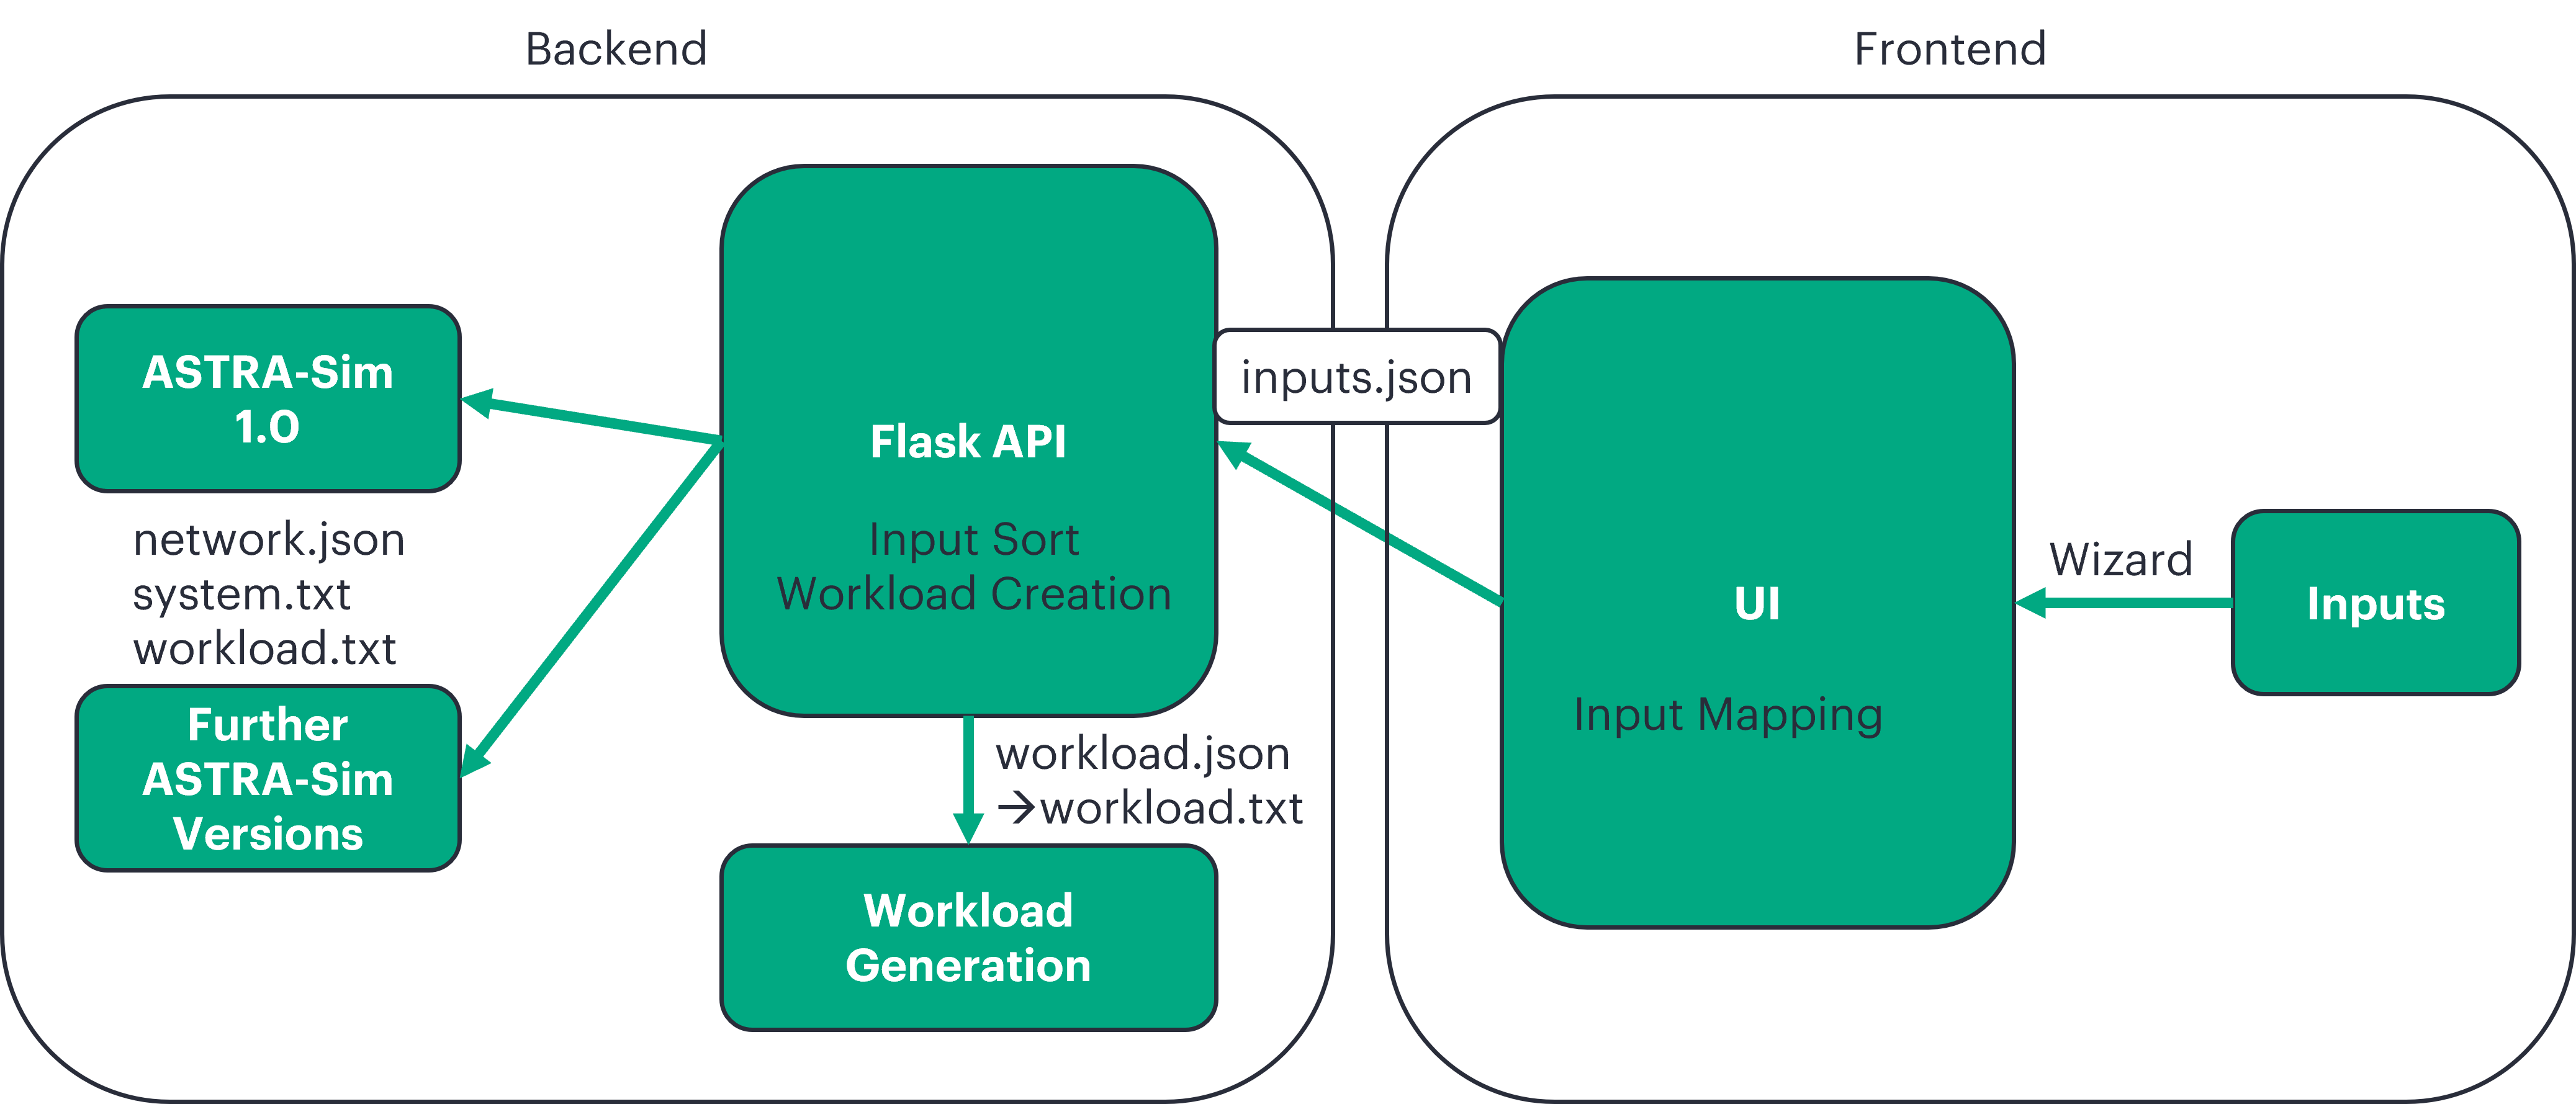
\includegraphics[width=1\textwidth]{api-architecture.png}
    \caption{General Structure Overview}
    \label{fig:architecture}
\end{figure}

The \ac{API} takes an input of one big \ac{JSON} file, that specifies all of \acp{ASTRA-Sim}' parameters. That allows retrieving the parameters form the frontend in a summed up way. Based on configurations depending on the \ac{ASTRA-Sim} version, different parameters for the three \textit{(or five)} input files can be specified. \\
The \ac{API} also takes the responsibility of generating the final wanted files. Because the different versions depend on varying input fields this can be adjusted in the backend by changing the algorithm of generating the files.
Also, the \ac{API} has access to a workload generation script, that takes inputs to generate workload files. Necessary inputs are retrieved from the suers choice of to be trained model. \\
Naturally, the frontend can support any structure of inputs and is not fixed to \ac{ASTRA-Sim} inputs with this data pipeline.
The frontend takes inputs from the user, here in form of a wizard and maps them to necessary \ac{ASTRA-Sim} inputs.



\section{Frontend Design}
% Wizard Handling (Data magic, wie aus eingaben andere weitergaben zu astra sim inputs werden)
% UI screenshot vs wireframe evtl evtl idk

% Figure \ref{fig:wire-4} shows the current implementation of the network page.
% One major difference to the previous designed wizard is that this one is not full page again. That design was chosen to awake the feeling that the wizard is integrated into the whole page and less an additional thing. In the end, this is the part where users might spend the most time.
% Another difference is, that the count of dimensions was integrated into the choice of physical topology. That way, the association between the count of dimensions and their actual existence gets more obvious for the user. 

% \begin{figure}[h]
%     \centering
%     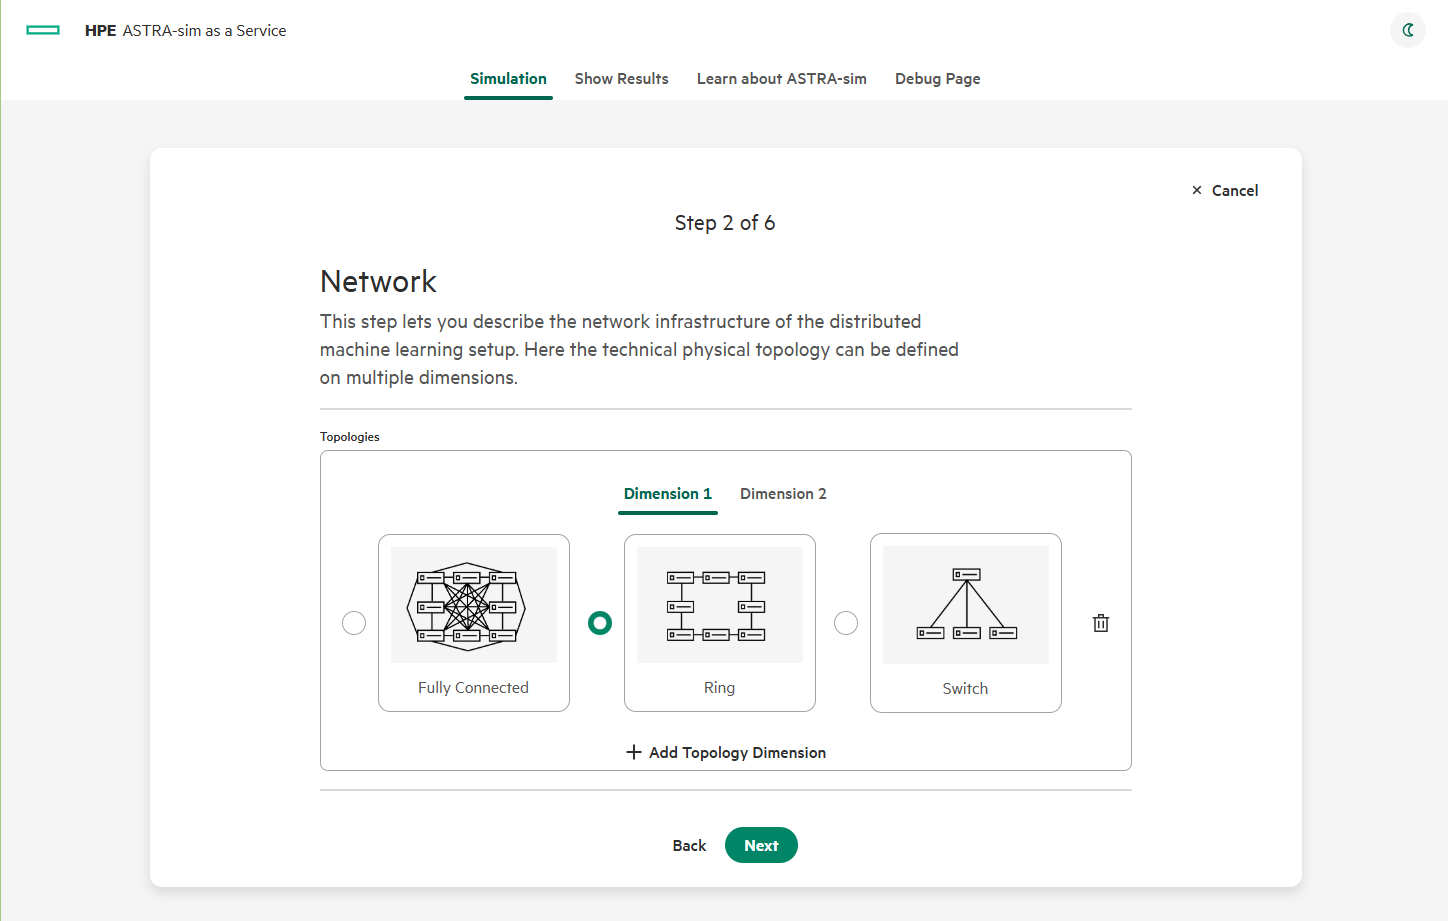
\includegraphics[width=0.75\textwidth]{implementation-network.png}
%     \caption{Final Implementation Network Page}
%     \label{fig:wire-4}
% \end{figure}

% Also, actual colors differentiate from the previous configurations, suiting current corporate branding suggestions. 



% \begin{figure}[H]
%     \centering
%     \includegraphics[width=0.8\textwidth]{figures/final_ui_screenshot.png}
%     \caption{Final UI screenshot}
% \end{figure}

\section{Backend Integration}
% ASTRA-Sim (Build in dockerfile + Aufruf in der Route)
% Parameter Einnahme sortieren & formatieren (zb von json to txt liste bei system file oder so den workload generator pfad)
% Error Handling
% Outputs

